\documentclass{article}

% if you need to pass options to natbib, use, e.g.:
%     \PassOptionsToPackage{numbers, compress}{natbib}
% before loading neurips_2020

% ready for submission
\usepackage[final]{neurips_2020}

% to compile a preprint version, e.g., for submission to arXiv, add add the
% [preprint] option:
%     \usepackage[preprint]{neurips_2020}

% to compile a camera-ready version, add the [final] option, e.g.:
%     \usepackage[final]{neurips_2020}

% to avoid loading the natbib package, add option nonatbib:
%\usepackage[nonatbib]{neurips_2020}

\usepackage[utf8]{inputenc} % allow utf-8 input
\usepackage[T1]{fontenc}    % use 8-bit T1 fonts
\usepackage{hyperref}       % hyperlinks
\usepackage{url}            % simple URL typesetting
\usepackage{booktabs}       % professional-quality tables
\usepackage{amsfonts}       % blackboard math symbols
\usepackage{nicefrac}       % compact symbols for 1/2, etc.
\usepackage{microtype}      % microtypography

\usepackage{graphicx}
\graphicspath{ {./figs/} }

\title{Randomized Overdrive Neural Networks}

% The \author macro works with any number of authors. There are two commands
% used to separate the names and addresses of multiple authors: \And and \AND.
%
% Using \And between authors leaves it to LaTeX to determine where to break the
% lines. Using \AND forces a line break at that point. So, if LaTeX puts 3 of 4
% authors names on the first line, and the last on the second line, try using
% \AND instead of \And before the third author name.

\author{%
  Christian J. ~Steinmetz \\
  Queen Mary University of London\\
  \texttt{c.j.steinmetz@qmul.ac.uk} \\
  \And
  Joshua D.~Reiss \\
  Queen Mary University of London \\
  \texttt{joshua.reiss@qmul.ac.uk} \\
}

\begin{document}

\maketitle

\begin{abstract}

By processing audio signals in the time-domain with randomly weighted temporal convolutional networks (TCNs),
we uncover a wide range of novel, yet controllable distortion and overdrive effects. 
We find that architectural aspects, such as the depth of the network, 
the kernel size, the number of channels, the activation function, as well as the weight initialization scheme, 
have a clear impact on the sonic character of the resultant effect, without the need for training. 
In practice, these effects range from relatively conventional overdrive effects,
to more extreme effects as the receptive field grows, akin to a fusion of distortion, equalization, delay, and reverb.  
To enable use by musicians and producers, we provide a real-time plugin implementation.
This allows users to dynamically design networks, listening to the to the results in real-time.
We provide a demo, along with builds at \url{https://ronn.ml}.

\end{abstract} 

% The TCN architecture can be viewed as a nonlinear waveshaper with memory
% equal to receptive field of the causal convolutional network. 

\section{Introduction}

Throughout the history of audio technology, engineers, circuit designers, 
and particularly guitarists, have searched for novel sonic effects as a result of clipping or distorting audio signals. 
These distortion effects were first discovered by pushing early guitar amplifiers beyond their operating range, 
or in some cases even from the accidental damage amplifiers or speakers \cite{shepherd2003distortion}. 
These pursuits are a clear example of creators taking advantage of the limitations of their tools for creative effect.
Today, distortion effects have permeated most genres like blues, jazz, rock, metal, 
and these effects also play a central roll in modern pop and hip-hop styles.
Whether it be vacuum tubes, diodes, transistors, op-amps, integrated circuits, or broken speaker drivers performing the distortion, 
it appears as if nearly all the methods of generating this sought after effect have been exhausted. 
But maybe there is a relatively under-explored in the task of generating distortion, and thats the realm of neural networks.

Neural networks are far from new, and in fact they arose in the same era that blues guitarists began their experiments with distortion \cite{schmidhuber2015deep}.
With the emergence of modern deep learning approaches, which have demonstrated the ability to tackle many modeling tasks in the audio domain,
these methods have already applied to the task of trying to mimic the characteristic distortion of famous amplifiers and distortion effects 
\cite{covert2013rnn, schmitz2018nonlinear, zhang2018lstm, damskagg2019distortion, martinez2019nonlinear}.
However, the aim of this work deviates from these modeling approaches.
Very much in the spirit of the original distortion pioneers, 
our work aims to take advantage of neural networks in a way that departs from their intended design, 
with the goal of. 

\cite{deman2014adaptive}
 
%\begin{figure}[h]
%  \centering
%  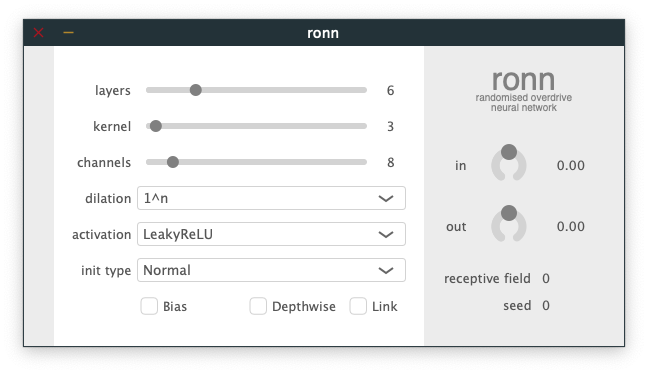
\includegraphics[width=0.7\textwidth]{ronn-vst-ui.png}
%\end{figure}

\section{Method}

\section{Discussion}

\section*{Broader Impact}

\section*{References}

\bibliography{references}{}
\bibliographystyle{plain}

\end{document}
